% A simple fault tree
% Author: Zhang Long, Mail: zhangloong[at]gmail.com
%\def\pgfsysdriver{pgfsys-dvipdfm.def}
\documentclass{minimal}
\usepackage{tikz}
\usepackage{verbatim}

\begin{comment}
:Title: Fault tree

A simple fault tree sample. "And" & "Or" gates shapes are from ``shapes.gates.logic.US`` library. Since they are all horizontal in the library, so they are rotated 90 degree before using.

First draw the tree without gates and other symbols like basic event symbol,  then place gates and symbols at the appropriate positions. Defining new "edge from parent path" rather than using "edge from parent fork down"  makes the branches nicer.

**Note**: The node labels are not correctly placed when using the CVS version of PGF. See comments in the source code for details.

\end{comment}
\usetikzlibrary{shapes.gates.logic.US,trees,positioning,arrows}
\begin{document}
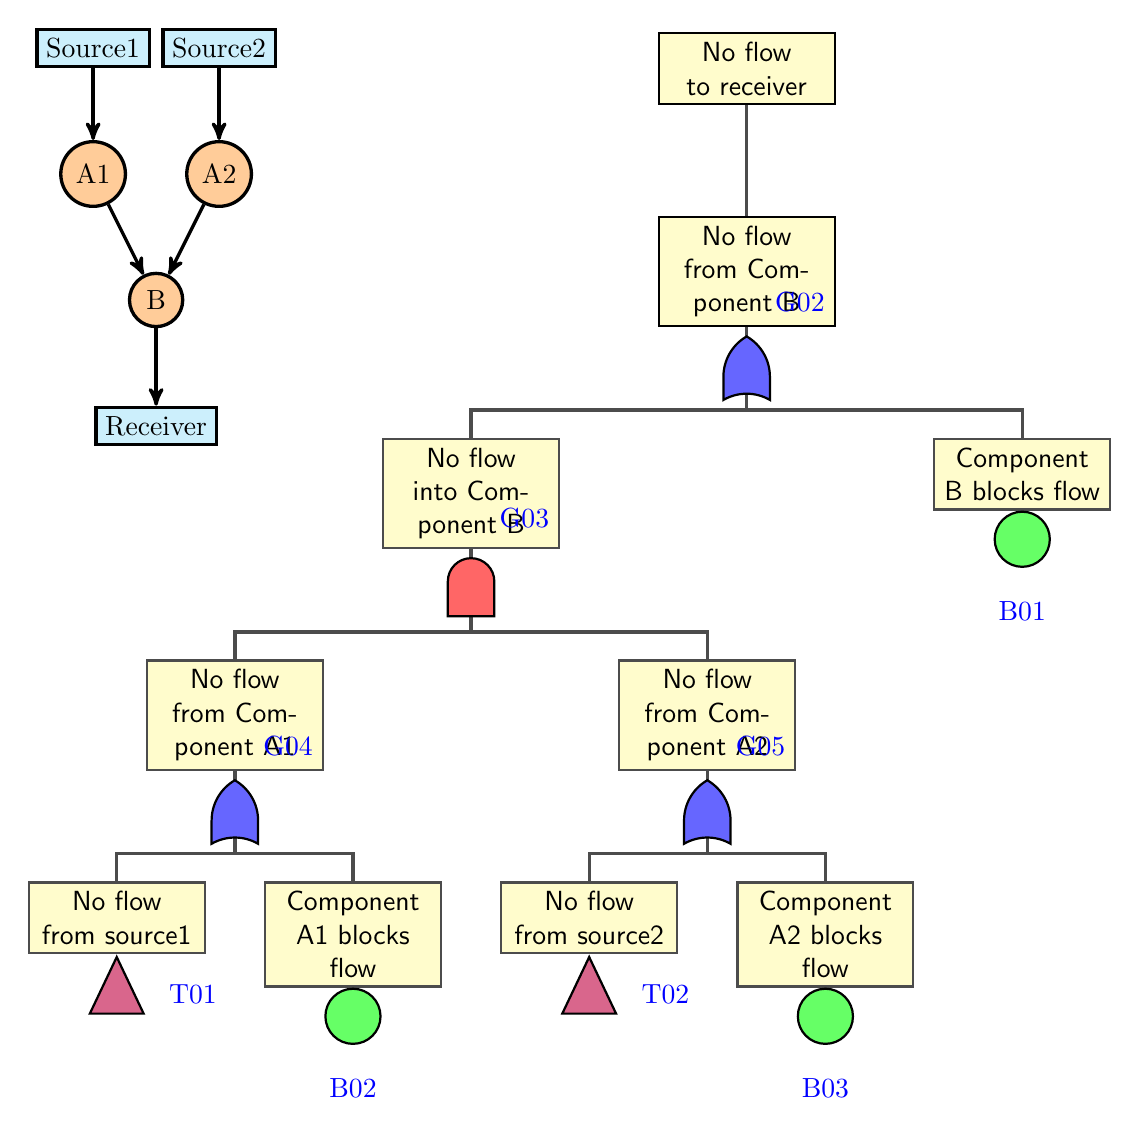
\begin{tikzpicture}[
% Gates and symbols style
    and/.style={and gate US,thick,draw,fill=red!60,rotate=90,
		anchor=east,xshift=-1mm},
    or/.style={or gate US,thick,draw,fill=blue!60,rotate=90,
		anchor=east,xshift=-1mm},
    be/.style={circle,thick,draw,fill=green!60,anchor=north,
		minimum width=0.7cm},
    tr/.style={buffer gate US,thick,draw,fill=purple!60,rotate=90,
		anchor=east,minimum width=0.8cm},
% Label style
    label distance=3mm,
    every label/.style={blue},
% Event style
    event/.style={rectangle,thick,draw,fill=yellow!20,text width=2cm,
		text centered,font=\sffamily,anchor=north},
% Children and edges style
    edge from parent/.style={very thick,draw=black!70},
    edge from parent path={(\tikzparentnode.south) -- ++(0,-1.05cm)
			-| (\tikzchildnode.north)},
    level 1/.style={sibling distance=7cm,level distance=1.4cm,
			growth parent anchor=south,nodes=event},
    level 2/.style={sibling distance=7cm},
    level 3/.style={sibling distance=6cm},
    level 4/.style={sibling distance=3cm}
%%  For compatability with PGF CVS add the absolute option:
%   absolute
    ]
%% Draw events and edges
    \node (g1) [event] {No flow to receiver}
	     child{node (g2) {No flow from Component B}   
	     	child {node (g3) {No flow into Component B}
	     	   child {node (g4) {No flow from Component A1}
	     	      child {node (t1) {No flow from source1}}
	     	      child {node (b2) {Component A1 blocks flow}}
			}
	     	   child {node (g5) {No flow from Component A2}
	     	      child {node (t2) {No flow from source2}}
	     	      child {node (b3) {Component A2 blocks flow}}
			}
		   }
	     	child {node (b1) {Component B blocks flow}}
		};
%% Place gates and other symbols
%% In the CVS version of PGF labels are placed differently than in PGF 2.0
%% To render them correctly replace '-20' with 'right' and add the 'absolute'
%% option to the tikzpicture environment. The absolute option makes the 
%% node labels ignore the rotation of the parent node. 
   \node [or]	at (g2.south)	[label=-20:G02]	{};
   \node [and]	at (g3.south)	[label=-20:G03]	{};
   \node [or]	at (g4.south)	[label=-20:G04]	{};
   \node [or]	at (g5.south)	[label=-20:G05]	{};
   \node [be]	at (b1.south)	[label=below:B01]	{};
   \node [be]	at (b2.south)	[label=below:B02]	{};
   \node [be]	at (b3.south)	[label=below:B03]	{};
   \node [tr]	at (t1.south)	[label=below:T01]	{};
   \node [tr]	at (t2.south)	[label=below:T02]	{};
%% Draw system flow diagram
   \begin{scope}[xshift=-7.5cm,yshift=-5cm,very thick,
		node distance=1.6cm,on grid,>=stealth',
		block/.style={rectangle,draw,fill=cyan!20},
		comp/.style={circle,draw,fill=orange!40}]
   \node [block] (re)					{Receiver};
   \node [comp]	 (cb)	[above=of re]			{B}  edge [->] (re);
   \node [comp]	 (ca1)	[above=of cb,xshift=-0.8cm]	{A1} edge [->] (cb);
   \node [comp]	 (ca2)	[right=of ca1]			{A2} edge [->] (cb);
   \node [block] (s1)	[above=of ca1]		{Source1} edge [->] (ca1);
   \node [block] (s2)	[right=of s1]		{Source2} edge [->] (ca2);
   \end{scope}
\end{tikzpicture}
\end{document}
